\listfiles
\documentclass[%
%prl%
%,preprint%
 ,twocolumn%
 ,secnumarabic%
%,tighte{docs}%
%\usepackage{bm}%
%\usepackage[colorlinks=true,linkcolor=blue]{hyperref}%
%\nofilesnlines%
,amssymb, amsmath,nobibnotes, aps, prl]{revtex4}
%\usepackage{acrofont}%NOTE: Comment out this line for the release version!
\usepackage
\expandafter\ifx\csname package@font\endcsname\relax\else
 \expandafter\expandafter
 \expandafter\usepackage
 \expandafter\expandafter
 \expandafter{\csname package@font\endcsname}%
\fi
\usepackage{t1enc} % as usual
\usepackage[utf8]{inputenc} % as usual
\usepackage{times}	
\usepackage{mathcomp}
\usepackage{amsmath}
\usepackage{graphicx}
\usepackage{subfigure}
\usepackage{hyperref}



\begin{document}

%Plan
%

\title{Coupling Impedance Bench Measurements of the Transverse Beam Coupling Impedance of Asymmetric Structures}

\author{Hugo Alistair Day}

\author{Elias Métral}
\author{Fritz Caspers}
\author{Benoit Salvant}
\author{Roger Jones}

\begin{abstract}
The analysis of data from the measurement of device impedance using the coaxial wire technique require a degree of understanding of both what is actually being measured by the method, and of what is being defined as a real and imaginary impedance. Through my own work I discovered a lack of clear definitions of how the data measured directly related to the quantities that we refer to from the point of view of particle motion. The idea of this document is to attempt to clarify how the quantities are related, and also give a clear guide as to how to analyse the experimental data to be compatible with a beam dynamics point of view. This presently a work in progress
\end{abstract}


\maketitle
\tableofcontents





% Introduction - Coaxial Wire Method
% Wakefield Basics - Definiton of longitudinal, dipolar/driving, quadrupolar/detuning impedance
% Analysis of transmission method
% Analysis of resonator method
%

\section{Introduction}
\label{sec:Intro}

Beam coupling impedance has been known as a driver of beam instabilities for some time [cite chao]. The ability to measure the beam impedance via the use of a bench top coaxial wire measuring technique has been used for a number of years, allowing the measurement of the longitudinal impedance [cite hahn/pedersen, sands/rees, vacarro, caspers], by using a single wire, and dipolar (or driving) transverse impedance[cite caspers], by use of two wires driven $\pi$ radians out of phase with one another,  of individual accelerator components. Recent work has proposed the use of a combination of a displaced single wire and two wire measurements to measure the quadrupolar (or detuning) impedance of structures with top/bottom, left/right symmetry [cite tsutsui-one-wire, metral et al PS MTE kicker]. 

In this paper we verify the proposed method for the measurement of the quadrupolar impedances in structures with top/bottom, left/right symmetry using simulated measurements of the coaxial wire measurements between a structure with two parallel plates. The formalism is subsequently extended to asymmetric structures, where it is demonstrated that it is possible to measure the quadrupolar and constant (not dependent on the displacement of the source or witness particle) transverse impedances of this type of structure. This method is then verified using simulated measurements of the method using an asymmetric structure for which an analytical model exists where excellent agreement is found for the real components of the longitudinal and transverse impedances and good agreement for the imaginary components.

The structure of the paper is as follows: Sec.~\ref{sec:coAxMeas} briefly introduces the physical reasoning behind using the coaxial measuring technique, in addition to a brief summary of the conversion from transmission parameters to beam impedance. In Sec.~\ref{sec:MathematicalFormalism} the formalism of the representation of the beam coupling impedance of a current carrying wire is introduced. In Secs.~\ref{sec:TopBotSymMath} and \ref{sec:TopBotSymSims} the method for analysing a structure with top/bottom, left/right symmetry is introduced (Sec.~\ref{sec:TopBotSymMath}) and demonstrated using a structure represented by two parallel plates (Sec.~\ref{sec:TopBotSymSims}). In Secs.~\ref{sec:AsymMath} and \ref{sec:AsymSims} the formalism is extended to cover asymmetric structures and then verified using simulations of coaxial wire measurements of an asymmetric structure, in this case a C-core ferrite kicker magnet. In Sec~\ref{sec:AsymSims} the results for the simulations are presented. In Sec.~\ref{sec:ConSum} the findings are summarised and the future steps for the work are proposed.

\section{Coaxial Wire Measurements of Beam Impedance}
\label{sec:coAxMeas}

A moving charged particle produces an electromagnetic field in a arc transverse to its direction of motion, where the angle of the arc opening is inversely proportional to the relativistic factor of the particle $\gamma$. For an ultrarelativistic particle ($\gamma \rightarrow \infty$), the field becomes entirely perpendicular to the direction of motion. If we place a conductive wire along the same path we would expect the charged particle to take (in most cases this is well represented by a straight wire), a short electrical pulse sent along this wire would propogate in the TEM (transverse electrical and magnetic field) mode, producing a field profile similar to that emitted by the ultrarelativistic charged particle (see. Fig. \ref{fig:coax-part-profile})

\begin{figure}
\begin{center}
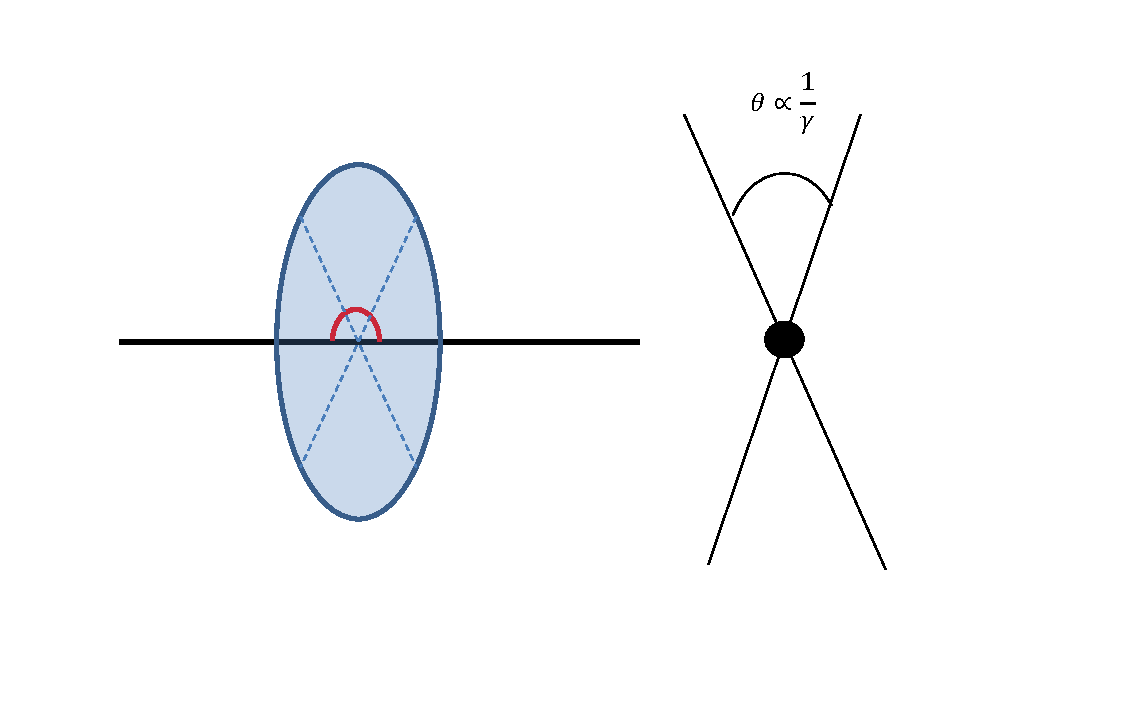
\includegraphics[width=0.6\textwidth]{figures/coaxial-particle-fields.pdf}
\end{center}
\caption{Comparison of the electromagnetic field profile of a moving charged particle and a short time pulse propagating along a coaxial wire.}
\label{fig:coax-part-profile}
\end{figure}

The value that we wish to measure to evaluate the beam coupling impedance of a device are the scattering parameters of the resulting circuit, in particular $S_{21}$, the normalised transmission parameter through the DUT. $S_{21}$ is calculated by taking the measured transmission parameter $S_{21,DUT}$ and dividing it by the transmission parameter through a reference line of the same physical length as the DUT,

\begin{equation}
S_{21} = \frac{S_{21,DUT}}{S_{21,REF}}.
\end{equation}

The effect of this is to correct the measured phase change in the DUT to be that only caused by the imaginary component of the beam coupling impedance.

There are subsequently a number of ways to evaluate the beam coupling impedance of the DUT depending on it's expected properties. For devices that are expected to have a either a small impedance, or those that are physically very short in length, it is possible to use the so called lumped impedance formula \cite{Hahn:BenchMeasInter, Hahn:ValidityImpMeas};

\begin{equation}
Z = 2Z_{c} \frac{1-S_{21}}{S_{21}}.
\end{equation}

For distributed impedances, it is suitable to use the so called log formula (called so due to attenuation causing a log function to appear in the evaluation) \cite{Hahn:BenchMeasInter, Hahn:ValidityImpMeas, Jensen:ImprovLogForm},

\begin{equation}
Z = -2Z_{c} ln \left( S_{21} \right).
\end{equation}

For long components or measurements at very high frequencies there exists the improved log formula. This takes into account more completely the electrical length of the device, given by

\begin{equation}
Z = -2Z_{c} ln \left( S_{21}  \right) \left( 1 + j\frac{ln \left( S_{21}\right) }{2\Theta}  \right)
\end{equation}

where $\Theta = 2\pi \frac{L}{\lambda}$ is the normalised electrical length of the device, $L$ the length of the device, $\lambda$ the wavelength of the frequency of measurement. It is possible to see that the lumped impedance formula can be used when $\Theta \leq 1$, and the improved log formula becomes useful for $\Theta \geq 5$ \cite{Jensen:ImprovLogForm}.

\section{Formalism of the Coaxial Wire in the Device Under Test}
\label{sec:MathematicalFormalism}

To derive the measurements required to allow the calculation of the transverse impedances of the measured device under test it is first necessary to consider the relationship of the beam impedance to be measured, and the current of the coaxial wire. First consider the general form of the $m$-th order ($m = 0, 1, 2,...$) longitudinal beam coupling impedance, given by \cite{Chao:PhysColEff, Tsutsui:OnSingleWire}

\begin{equation}
\bar{Z}_{m} = \frac{-1}{I^{2}} \int dV \mathbf{\bar{E}_{m}. \bar{J}_{m}^{*}}
\end{equation}

where $\bar{J}_{m}$ is the current density of the source. For a beam propogating along the z-axis with an offset $a$ and moment $cos \left( m \theta \right)$,

\begin{equation}
\mathbf{\bar{J}_{m}} = \frac{I}{\pi a^{m +1} \left( 1 + \delta_{m0} \right)} \delta \left( r - a \right) cos \left( m \theta \right) exp \left( j \left( \omega t - k z  \right) \right) \mathbf{e_{z}}.
\end{equation}

The electromagnetic field associated with a given current source $\mathbf{\bar{J}_{m}}$ is $\left( \mathbf{\bar{E}_{m}}, \mathbf{\bar{H}_{m}} \right)$. 

It can be seen that any different azimuthal components of the $m$-th field of order $n$ (i.e. $sin \left( n\theta \right)$ and $cos \left( n\theta \right)$ terms) are neglected in this treatment. To allow the treatment of coupling between different azimuthal orders we can define a longitudinal beam coupling impedance $Z_{m,n}$ (where $m,n = 0, \pm 1, \pm 2, ... $)

\begin{equation}
Z_{m,n} = \frac{-1}{I^{2}} \int dV \mathbf{E_{m}. J_{n}^{*}}
\end{equation}

where

\begin{equation}
\mathbf{J_{m}} = \frac{I}{2 \pi a^{|m |+1}} \delta \left( r - a \right) exp \left(j m \theta \right) exp \left( j \left( \omega t - k z  \right) \right) \mathbf{e_{z}}.
\end{equation}

Importantly, this allows us to see that 

\begin{align}
\mathbf{\bar{J}_{0}} &= \mathbf{J_{0}} \nonumber \\
\mathbf{\bar{J}_{m}} &= \mathbf{J_{m}} + \mathbf{J_{-m}}.
\end{align}

From here we use the principle of superposition for electromagnetic fields (i.e. we neglect any non-linearities of the surrounding materials), and thus can derive

\begin{align}
\bar{Z}_{0} &= Z_{0} \\
\bar{Z}_{x} &= \bar{Z}_{1} = Z_{1,1} + Z_{1,-1} + Z_{-1,1} + Z_{-1,-1} = kZ^{dip}_{x}\\
\bar{Z}_{x} &= \bar{Z}_{1} \text{(cos replaced with sin)}= Z_{1,1} - Z_{1,-1} - Z_{-1,1} + Z_{-1,-1} = kZ^{dip}_{y}\\
\bar{Z}_{m} &= Z_{m,m} + Z_{m,-m} + Z_{-m,m} + Z_{-m,-m}, m=1,2,...
\end{align}

From this start we will apply this to both two wire measurements and to displaced single wire measurements.

\subsubsection{Two Wire Measurements}

It is possible to directly measure the dipolar impedance of a device through the use of a two wire coaxial method. The measurement setup is identical to that of the single wire method, except that two wires, seperated by distance $\Delta$, are placed in the device, and a 180$^{\circ}$ hybrid is place between the wires and the VNA at both ends of the device. This setup is illustrated in Fig. \ref{fig:two_wire_measure}

\begin{figure}
\begin{center}
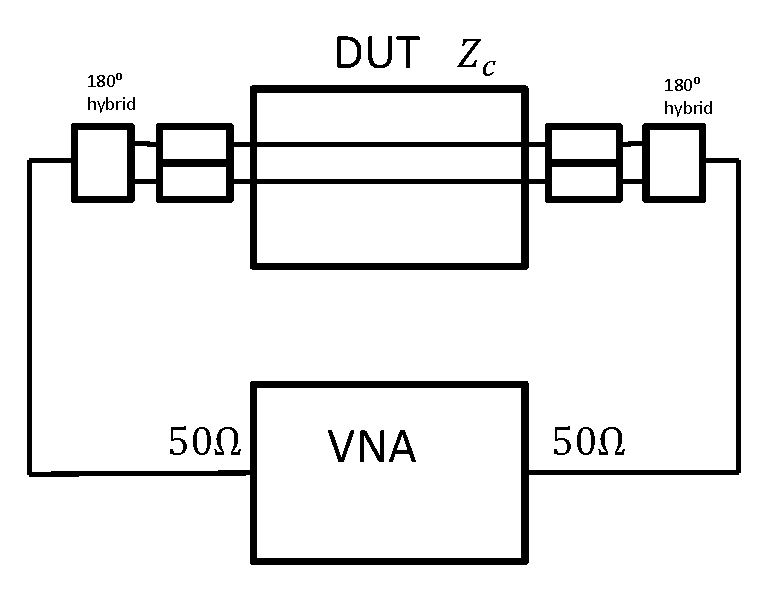
\includegraphics[width=0.6\textwidth]{figures/wire_meas_two_wire.pdf}
\end{center}
\caption{Measurement setup for measurements of the dipolar beam coupling impedance using the two wire setup for the classical coaxial wire method.}
\label{fig:two_wire_measure}
\end{figure}

As with the single wire measurements the transmission parameter is measured. Both wires are individually matched to $Z_{c}$. By using two wires each carrying a signal $\pi$ out of phase with one another we produce a field pattern similar to a dipole and thus measure the dipole impedance in either the horizontal or vertical plane depending on the orientation of the two wires. 

What is directly measured is the longitudinal impedance of just the dipole impedance, as is to be expected from the Panofsky-Wenzel theorem [cite Walling, Nassibian and Sacherer]. 

For two wire placed as positions $x = \pm a$, the current density is given by \cite{Tsutsui:OnSingleWire}

\begin{align}
J & =  I \left( \delta \left( x - a \right) - \delta \left( x + a  \right) \right) \delta (y) exp \left( j \left( \omega t - kz \right) \right) \nonumber \\
& =  \frac{I}{\pi a} \displaystyle\sum\limits_{m=-\infty}^{\infty} exp \left(j \left( 2m +1 \right) \theta \right) exp \left( j \left( \omega t - kz \right) \right) \nonumber \\
& =  2\displaystyle\sum\limits_{m=-\infty}^{\infty} a^{|2m + 1 |} J_{2m + 1}.
\end{align}

The impedance is then

\begin{align}
Z & =  - \frac{1}{I^{2}} \int dV \left( 2\displaystyle\sum\limits_{m=-\infty}^{\infty} a^{|2m + 1 |} E_{2m + 1}  \right)  \left( 2\displaystyle\sum\limits_{n=-\infty}^{\infty} a^{|2n + 1 |} J_{2n + 1}^{*}  \right) \nonumber \\
& =  4 \displaystyle\sum\limits_{m,n} a^{|2m + 1 | + |2n + 1|} Z_{2m + 1, 2n+1} \nonumber \\
& =  \left(2a \right)^{2}\left( Z_{1,1} + Z_{-1,1} + Z_{1,-1} + Z_{-1,-1} \right) + O(a^{4}) \nonumber \\
& =  (2a)^{2}\bar{Z}_{x} + O(a^{4}). 
\end{align}

Again using the Panofsky-Wenzel theorem we can deduce that the transverse dipolar impedance $Z^{dip}_{x/y}$ is given by 

\begin{equation}
Z^{dip}_{x/y} = \frac{\bar{Z}_{x/y}}{k} = \frac{c}{\omega} \frac{Z}{\Delta^{2}}
\end{equation}

where $\Delta = 2a$ and $Z$ is the measured complex impedance.

\section{The Impedance of a Displaced Coaxial Wire in a Device with top/bottom, left/right Symmetry}
\label{sec:TopBotSymMath}

If we consider a source particle at at $x_{1} = a_{1}cos\theta_{1}, y_{1} = a_{1}sin\theta_{1}$ and a test particle at $x_{2} = a_{2}cos\theta_{2}, y_{2} = a_{2}sin\theta_{2}$, the source current density is

\begin{align}
J_{z} &= I\delta \left( x-x_{1} \right) \delta \left( y-y_{1} \right) exp \left( k \left( \omega t - kz \right) \right) \nonumber \\
          &=\displaystyle\sum\limits_{m=-\infty}^{\infty}a_{1}^{|m|}exp\left( -jm\theta_{1} \right) J_{m}
\end{align}

The impedance would therefore be

\begin{align}
Z = &\frac{-1}{I^{2}} \int dV \left( \displaystyle\sum\limits^{\infty}_{m=-\infty} a_{1}^{|m|} exp \left( jm\theta_{1} \right) E_{m}\right) \left( \displaystyle\sum\limits^{\infty}_{n=-\infty} a_{1}^{|n|} exp \left( jn\theta_{2} \right) J^{*}_{n}\right) \nonumber \\
   = &\displaystyle\sum\limits^{\infty}_{m,n=-\infty} a_{1}^{|m|} a_{2}^{|n|} exp\left( -jm\theta_{1} \right) exp\left( -jn\theta_{2} \right) Z_{m,n} \nonumber \\
   = &Z_{0,0} + \left( x_{1}- jy_{1} \right)Z_{1,0} + \left( x_{1} + jy_{1} \right)Z_{-1,0} + \left( x_{2} + jy_{2} \right)Z_{0,1} +  \left( x_{2} - jy_{2} \right)Z_{0,-1} \nonumber \\
      & +\left( x_{1} - jy_{1} \right)^{2}Z_{2,0} +  \left( x_{1} - jy_{1} \right)\left( x_{2} - jy_{2} \right)Z_{1,-1} + \left( x_{2} - jy_{2} \right) Z_{0,-2} \nonumber \\
      & +\left( x_{1} - jy_{1} \right)\left( x_{2} + jy_{2} \right)Z_{1,1} + \left( x_{1} + jy_{1} \right) \left( x_{2} - jy_{2} \right) Z_{-1,-1} \nonumber \\
      & +\left( x_{1} + jy_{1} \right)^{2}Z_{-2,0} + \left( x_{1} + jy_{1} \right)\left( x_{2} - jy_{2} \right) Z_{-1,1} + \left( x_{2} - jy_{2} \right)^{2}Z_{0,2} \nonumber \\
      & +O\left( \left(  x_{1},y_{1},x_{2},y_{2} \right)^{3} \right).
\label{eqn:gen_imp}
\end{align}

By applying Panofsky-Wenzel we see

\begin{align}
kZ_{x} =\frac{\partial Z}{\partial x_{2}} = & Z_{0,1} + Z_{0,-1} + \left( x_{1} - jy_{1} \right) Z_{1,-1} + 2\left( x_{2} - jy_{2} \right) Z_{0,-2} \nonumber \\
						&+ \left( x_{1} - jy_{1} \right) Z_{1,1} + \left( x_{1} + jy_{1} \right) Z_{-1,-1} + \left( x_{1} + jy_{1} \right) Z_{-1,1} + 2\left( x_{2} + jy_{2} \right) Z_{0,2} \nonumber \\
						& + O\left( \left( x_{1},y_{1},x_{2},y_{2} \right)^{2} \right) \nonumber \\
						= & Z_{0,1} + Z_{0,-1} + x_{1}\bar{Z}_{x} + jy_{1} \left( -Z_{1,-1} - Z_{1,1} + Z_{-1,-1} + Z_{-1,1} \right) \nonumber \\
						& + x_{2}\left( 2Z_{0,-2} + 2Z_{0,2}  \right) + jy_{2}\left( -2Z_{0,-2} + 2Z_{0,2}  \right) +  O\left( \left( x_{1},y_{1},x_{2},y_{2} \right)^{2} \right)
\end{align}

\begin{align}
kZ_{y} =\frac{\partial Z}{\partial y_{2}} = & jZ_{0,1} - jZ_{0,-1} - j\left( x_{1} - jy_{1} \right) Z_{1,-1} - 2j\left( x_{2} - jy_{2} \right) Z_{0,-2} \nonumber \\
						&+ j\left( x_{1} - jy_{1} \right) Z_{1,1} - j\left( x_{1} + jy_{1} \right) Z_{-1,-1} + j\left( x_{1} + jy_{1} \right) Z_{-1,1} + 2j\left( x_{2} + jy_{2} \right) Z_{0,2} \nonumber \\
						& + O\left( \left( x_{1},y_{1},x_{2},y_{2} \right)^{2} \right) \nonumber \\
						= & j\left(Z_{0,1} - Z_{0,-1} \right)+ y_{1}\bar{Z}_{y} + jx_{1} \left( -Z_{1,-1} + Z_{1,1} + Z_{-1,-1} + Z_{-1,1} \right) \nonumber \\
						& + y_{2}\left(- 2Z_{0,-2} - 2Z_{0,2}  \right) + jx_{2}\left( -2Z_{0,-2} + 2Z_{0,2}  \right) +  O\left( \left( x_{1},y_{1},x_{2},y_{2} \right)^{2} \right).
\end{align}

Two properties to note for later use are that

\begin{align}
\textbf{J}_{-m} \left( \omega \right) & = \textbf{J}_{m}^{*} \left( -\omega \right) \\
Z_{-m,-n} \left( \omega \right) & = Z_{m,n}^{*} \left( -\omega \right).
\end{align}

If we now assume a single wire rather than a source and test particle, such that $x_{1}=x_{2}=x_{0}, y_{1}=y_{2}=y_{0}$. This gives a source current density

\begin{align}
J & = I \delta \left( x-x_{0} \right)\delta \left( y-y_{0} \right) exp\left( j \left(\omega t -kz \right)\right) \nonumber \\
  & = \frac{I}{2\pi a} \delta \left( r-a \right)\displaystyle\sum\limits_{m=-\infty}^{\infty} exp\left( jm \left( \theta -\theta_{0} \right) \right) exp\left( jm \left( \theta -\theta_{0} \right) \right) exp\left( j \left( \omega t - kz \right) \right) \nonumber \\
  & = \displaystyle\sum\limits_{m=-\infty}^{\infty} a^{|m|}exp\left( -jm\theta_{0} \right)J_{m}.
\end{align}

We can then define $x_{0}=acos\theta_{0}, y_{0}=asin\theta_{0}$. Entering this into Eqn. \ref{eqn:gen_imp} gives

\begin{align}
Z &=&Z_{0,0} +  \left( x_{0} - jy_{0} \right) Z_{1,0} + \left( x_{0} + jy_{0} \right)  Z_{-1,0} + \left( x_{0} + jy_{0} \right) Z_{0,1} \nonumber \\
   &   &+ \left( x_{0} - jy_{0} \right) Z_{0,-1} + \left( x_{0} - jy_{0} \right)^{2} Z_{2,0} + \left( x_{0} - jy_{0} \right)^{2} Z_{1,-1} + \left( x_{0} - jy_{0} \right) ^{2}Z_{0,-2} \nonumber \\
   &   &+\left( x_{0} - jy_{0} \right) \left( x_{0} + jy_{0} \right) Z_{1,1} + \left( x_{0} + jy_{0} \right)\left( x_{0} - jy_{0} \right) Z_{-1,-1} + \left( x_{0} + jy_{0} \right)^{2}Z_{-2,0} \nonumber \\
   &   &+\left( x_{0} + jy_{0} \right)^{2} Z_{-1,1} + \left( x_{0} + jy_{0} \right)^{2}Z_{0,2} + O\left( \left(x_{0},y_{0} \right)^{2} \right) \nonumber \\
   &=&Z_{0,0} + x_{0}\left( Z_{1,0}+Z_{-1,0}+Z_{0,1}+Z_{0,-1} \right) +jy_{0} \left( -Z_{-1,0} + Z_{-1,0} + Z_{0,1} - Z_{0,-1} \right) \nonumber \\
   &   &+x_{0}^{2} \left(  Z_{1,-1}+Z_{1,1}+Z_{-1,-1}+Z_{-1,1} + Z_{2,0} + Z_{0,-2} + Z_{0,2} + Z_{-2,0} \right) \nonumber \\
   &   &+y_{0}^{2} \left(  -Z_{1,-1}+Z_{1,1}+Z_{-1,-1}-Z_{-1,1} - Z_{2,0} - Z_{0,-2} - Z_{0,2} - Z_{-2,0} \right) \nonumber \\
   &   &+2jx_{0}y_{0}\left( -Z_{2,0} - Z_{0,-2} + Z_{-2,0} + Z_{0,2} + Z_{-1,1} - Z_{1,-1} \right) \nonumber \\
   &=&Z_{0,0} + x_{0}\left( Z_{1,0}+Z_{-1,0}+Z_{0,1}+Z_{0,-1} \right) +jy_{0} \left( -Z_{-1,0} + Z_{-1,0} + Z_{0,1} - Z_{0,-1} \right) \nonumber \\
   &   &+x_{0}^{2} \left( \bar{Z}_{x} + Z_{2,0} + Z_{0,-2} + Z_{0,2} + Z_{-2,0} \right) \nonumber \\
   &   &+y_{0}^{2} \left( \bar{Z}_{y} - Z_{2,0} - Z_{0,-2} - Z_{0,2} - Z_{-2,0} \right) \nonumber \\
   &   &+2jx_{0}y_{0}\left( -Z_{2,0} - Z_{0,-2} + Z_{-2,0} + Z_{0,2} + Z_{-1,1} - Z_{1,-1} \right).
\label{eqn:gen_single_wire}
\end{align}

It can then be seen that if measurements are made with $x_{0} = 0$ and taking different values of $y_{0}$ that one obtains data with a parabolic fit in the $y_{0}$ axis. By fitting a curve to this we obtain constant (equal to the longitudinal impedance), linear and quadratic terms. Doing the same for $y_{0}=0$ allows us to derive two quadratic terms

\begin{align}
Z^{\perp}_{x} & = \left( \bar{Z}_{x} + kZ_{quad} \right)\frac{1}{k} =  Z^{dip}_{x} + kZ_{quad}\\
Z^{\perp}_{y} & = \left( \bar{Z}_{y} - kZ_{quad} \right)\frac{1}{k}= Z^{dip}_{y} - kZ_{quad} \\
\end{align}

where $Z_{quad}=\frac{1}{k}\left( Z_{0,2}+Z_{2,0}+Z_{0,-2}+Z_{-2,0}  \right) = \frac{2}{k}\left( Z_{0,2}+Z_{0,-2}  \right)$, representing the impedance due to the displacement of the test particle in an accelerator. As we can measure $\bar{Z}_{x/y}$ independently using the two wire method we can thus indepedently measure $Z_{quad}$ using a displaced single wire scan in both the x- and y-planes.

It can also be seen that

\begin{align}
Z^{\perp}_{x} + Z^{\perp}_{y} = \frac{1}{k}\left( \bar{Z}_{x} + \bar{Z}_{y} \right) = Z^{dip}_{x} + Z^{dip}_{y}
\end{align}

where $\bar{Z}_{x/y}$ can be measured independently which gives a method of obtaining confidence in the wire measurements.



\section{Simulated Measurements of Coaxial Wire Technique between two Parallel Plates}
\label{sec:TopBotSymSims}

\begin{figure}
\begin{center}
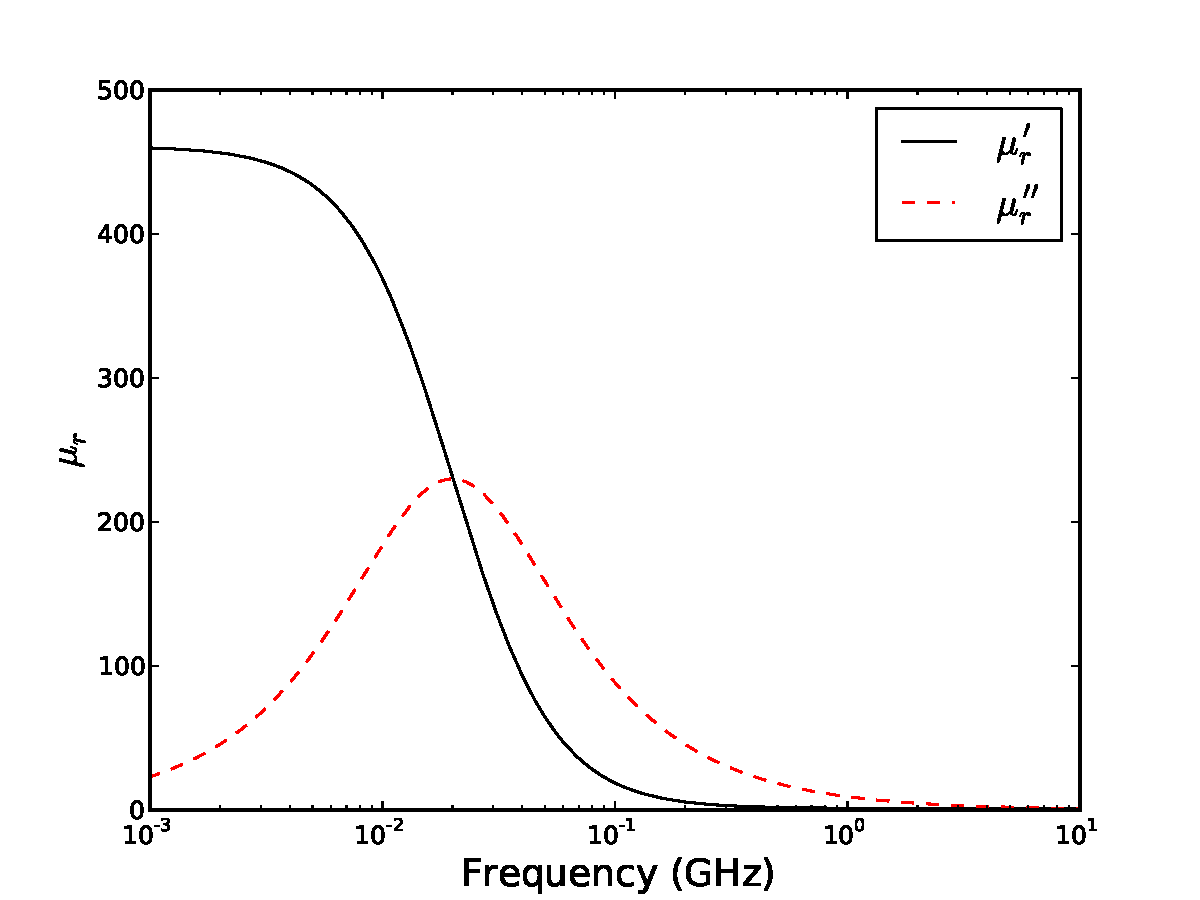
\includegraphics[width=0.45\textwidth]{figures/4A4FerrMu.pdf}
\end{center}
\caption{The complex permeability of 4A4 ferrite.}
\label{fig:4a4permeability}
\end{figure}

\begin{figure}
\begin{center}
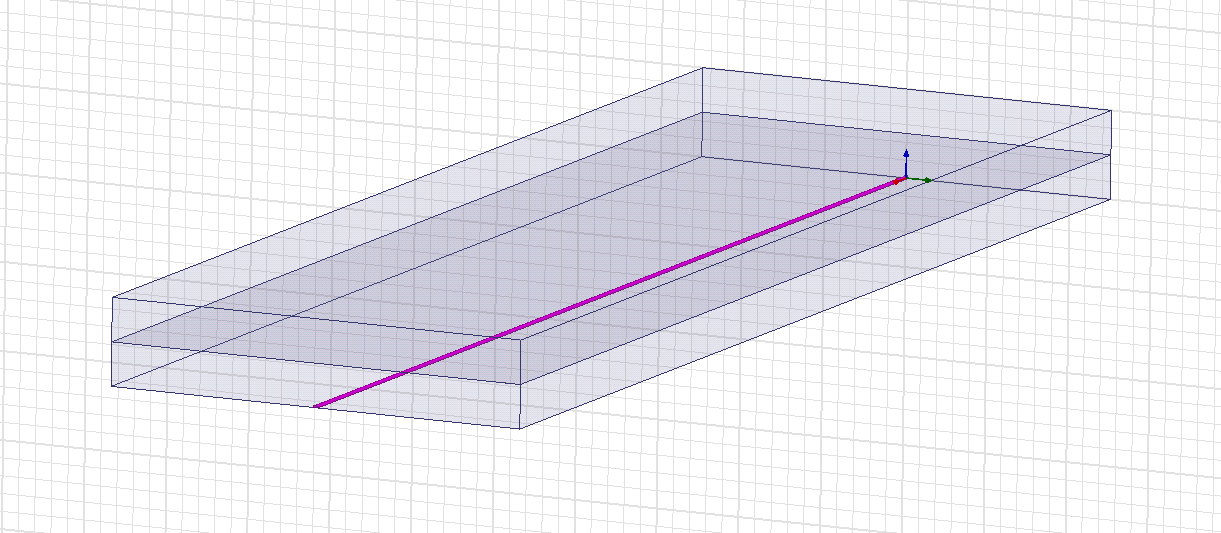
\includegraphics[width=0.5\textwidth]{figures/cross-section-coaxial-wire-measurements.png}
\end{center}
\caption{An example of the simulation model used for coaxial wire simulations. In this case a displaced single wire between two ferrite plates. The wire is highlighted in purple.}
\label{fig:wire-sim-model}
\end{figure}

For the simulations of a structure with top/bottom, left/right symmetry a structure comprised of two parallel ferrite plates is measured. For the simulated measurements the frequency domain code HFSS [hfss cite] is used. This allows the definition of waveguide ports on extremities of the measured structure (shown in Fig.~\ref{fig:wire-sim-model} where a half structure is used) and the measurement transmission parameters between the two waveguide ports. This allows the automatic matching of the structure removing the reflections due to the connection to the external circuit present in physical measurements. 

In this simulations the ferrite used is modelled on the 4A4 ferrite, the permitivitty of which is $\epsilon^{'} = 10$, and the frequency dependent permeability given in Fig.~\ref{fig:4a4permeability}. The conductivity is $\sigma_{4A4} = 10^{-6} S m^{-1}$, usual for vacuum ferrites to prevent electrostatic build up.

For these simulations the following parameters were used; for the displaced single wire measurements a wire of 0.3mm in radius, and the following displacement used to acquire the total transverse terms:

\begin{enumerate}
\item{In the horizontal axis -  displaced between -6mm to +6mm at intervals of 2mm}
\item{In the vertical axis - displaced between -4mm to +4mm at intervals of 2mm.}
\end{enumerate}

For the two wire simulations, two wires of radius 0.3mm are used, with a seperation of 4mm in the x-dimension, and 3mm in the y-dimension. 4 simulation configurations are used described below:

\begin{enumerate}
\item{an adaptive mesh generation set to a convergence criteria of $S_{21}$ diverging by less than 0.005 between two subsequent solutions, at an adaptive frequency of 20MHz solving to a second order basis. A discrete frequency sweep is then carried out in the range 1-10MHz at 1MHz intervals.}
\item{an adaptive mesh generation set to a convergence criteria of $S_{21}$ diverging by less than 0.005 between two subsequent solutions, at an adaptive frequency of 200MHz solving to a second order basis. A discrete frequency sweep is then carried out in the range 10-100MHz at 10MHz intervals.}
\item{an adaptive mesh generation set to a convergence criteria of $S_{21}$ diverging by less than 0.005 between two subsequent solutions, at an adaptive frequency of 2GHz solving to a second order basis. A discrete frequency sweep is then carried out in the range 100MHz-1GHz at 100MHz intervals.}
\item{an adaptive mesh generation set to a convergence criteria of $S_{21}$ diverging by less than 0.005 between two subsequent solutions, at an adaptive frequency of 10GHz solving to a second order basis. A discrete frequency sweep is then carried out in the range 1-10GHz at 1GHz intervals.}
\end{enumerate}

These parameters are used to benefit from an appropriate mesh count for the given frequency range, thus increasing simulation speed by not using a high density mesh at frequencies where no benefits would be gained.

\begin{figure}
\subfigure[]{
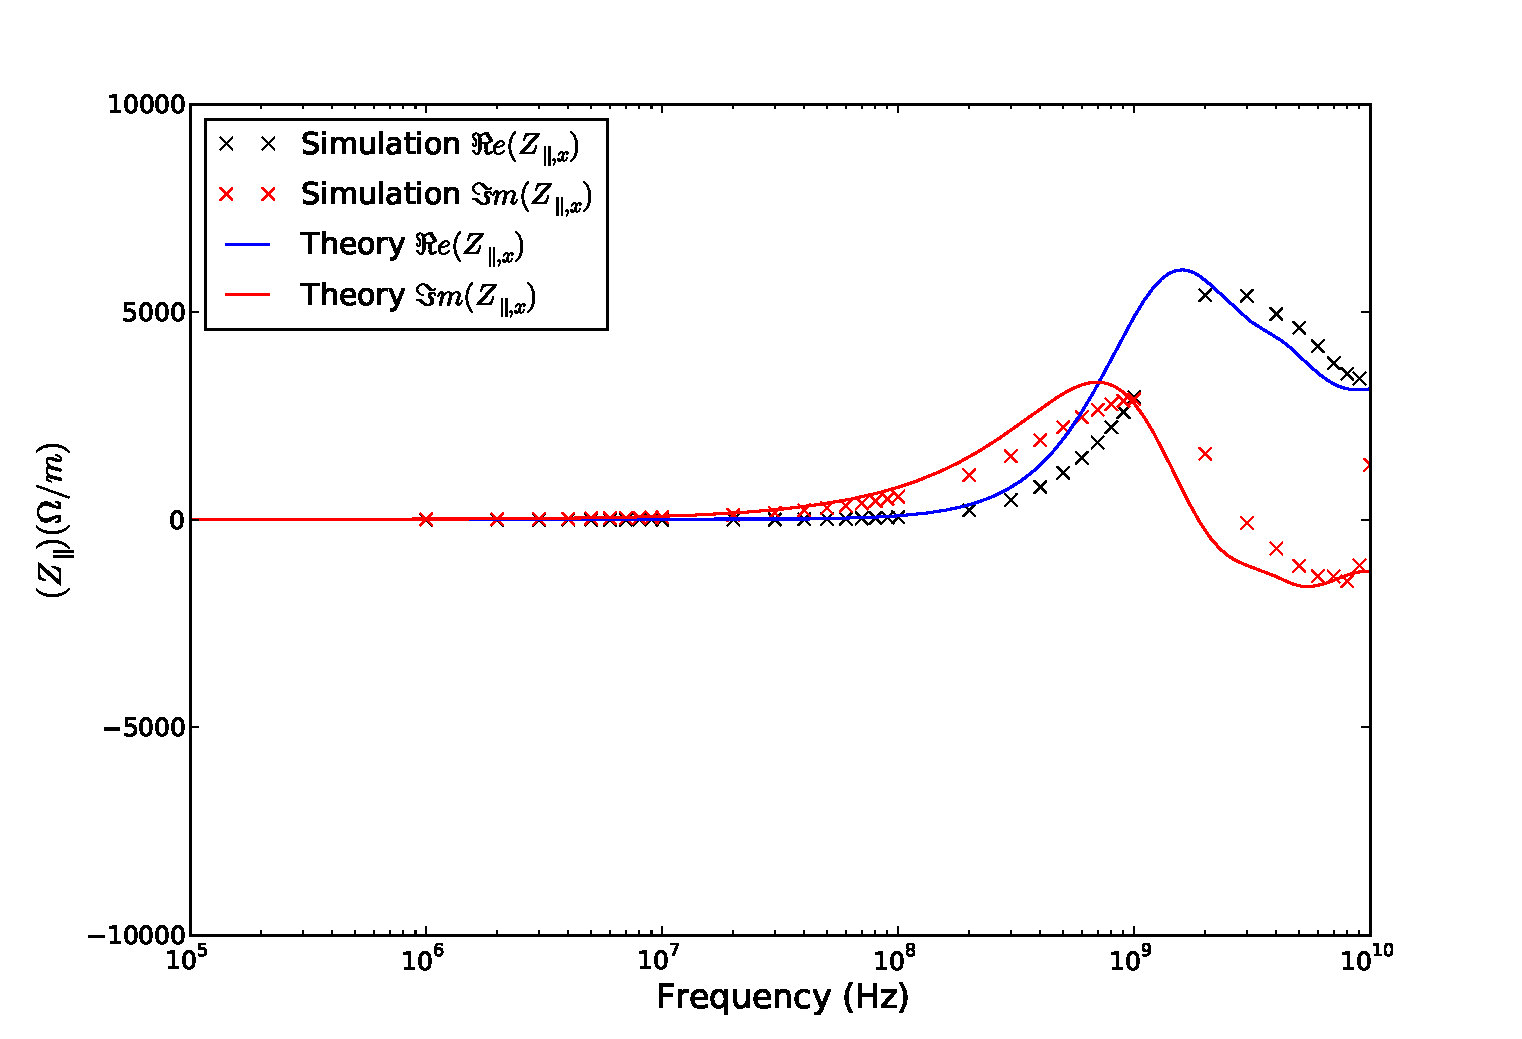
\includegraphics[width=0.5\textwidth]{figures/wire_meas/ferrite_plates/longitudinal-horizontal.pdf}
\label{fig:ferrite-plates-long-horz}
}
\subfigure[]{
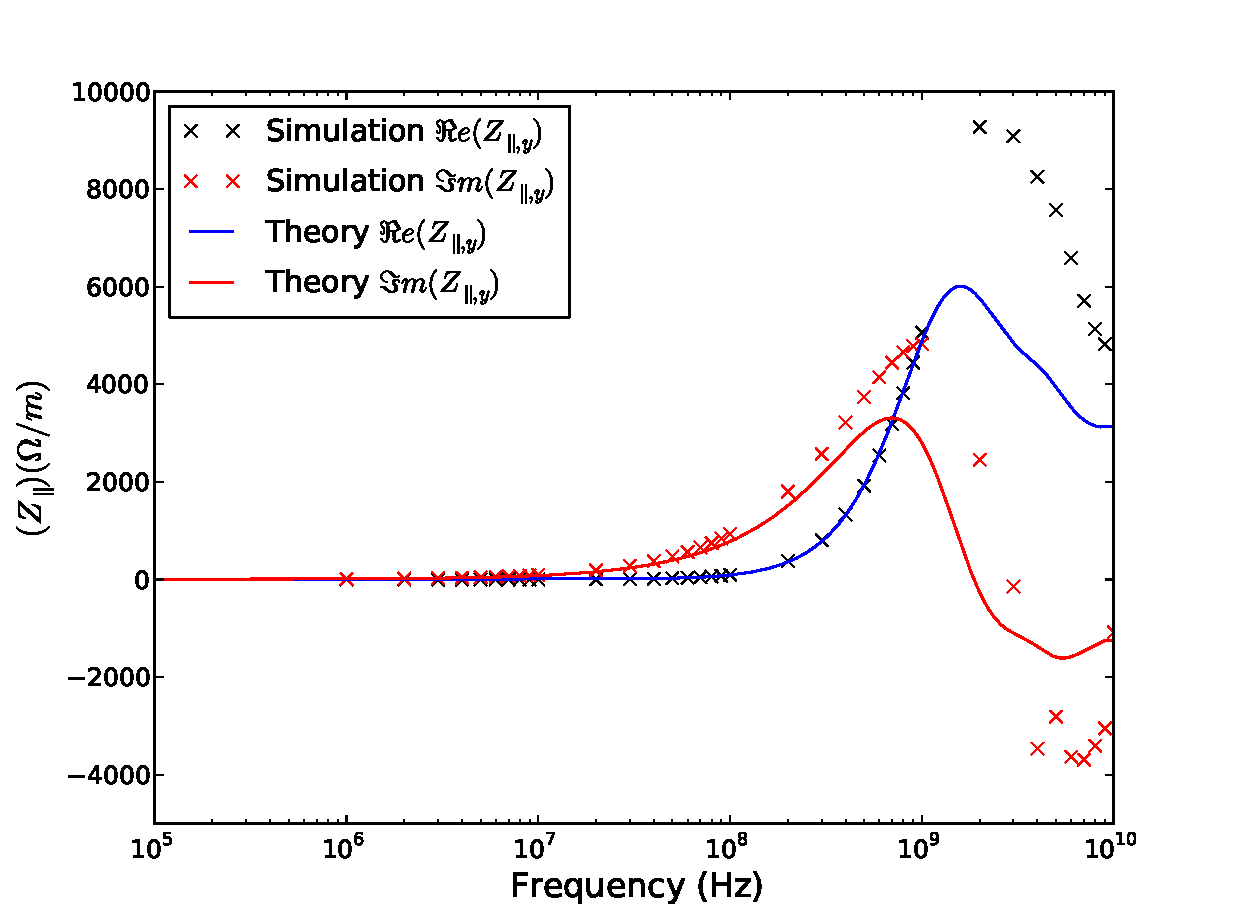
\includegraphics[width=0.5\textwidth]{figures/wire_meas/ferrite_plates/longitudinal-vertical.pdf}
\label{fig:ferrite-plates-long-vert}
}
\caption{The longitudinal impedance of two parallel ferrite plates simulated using a longitudinal coaxial wire. Presented are is the impedance as measured in the horizontal plane (\ref{fig:ferrite-plates-long-horz}) and in the vertical plane \ref{fig:ferrite-plates-long-vert}.}
\label{fig:ferrite-plates-long}
\end{figure}

\begin{figure}
\subfigure[]{
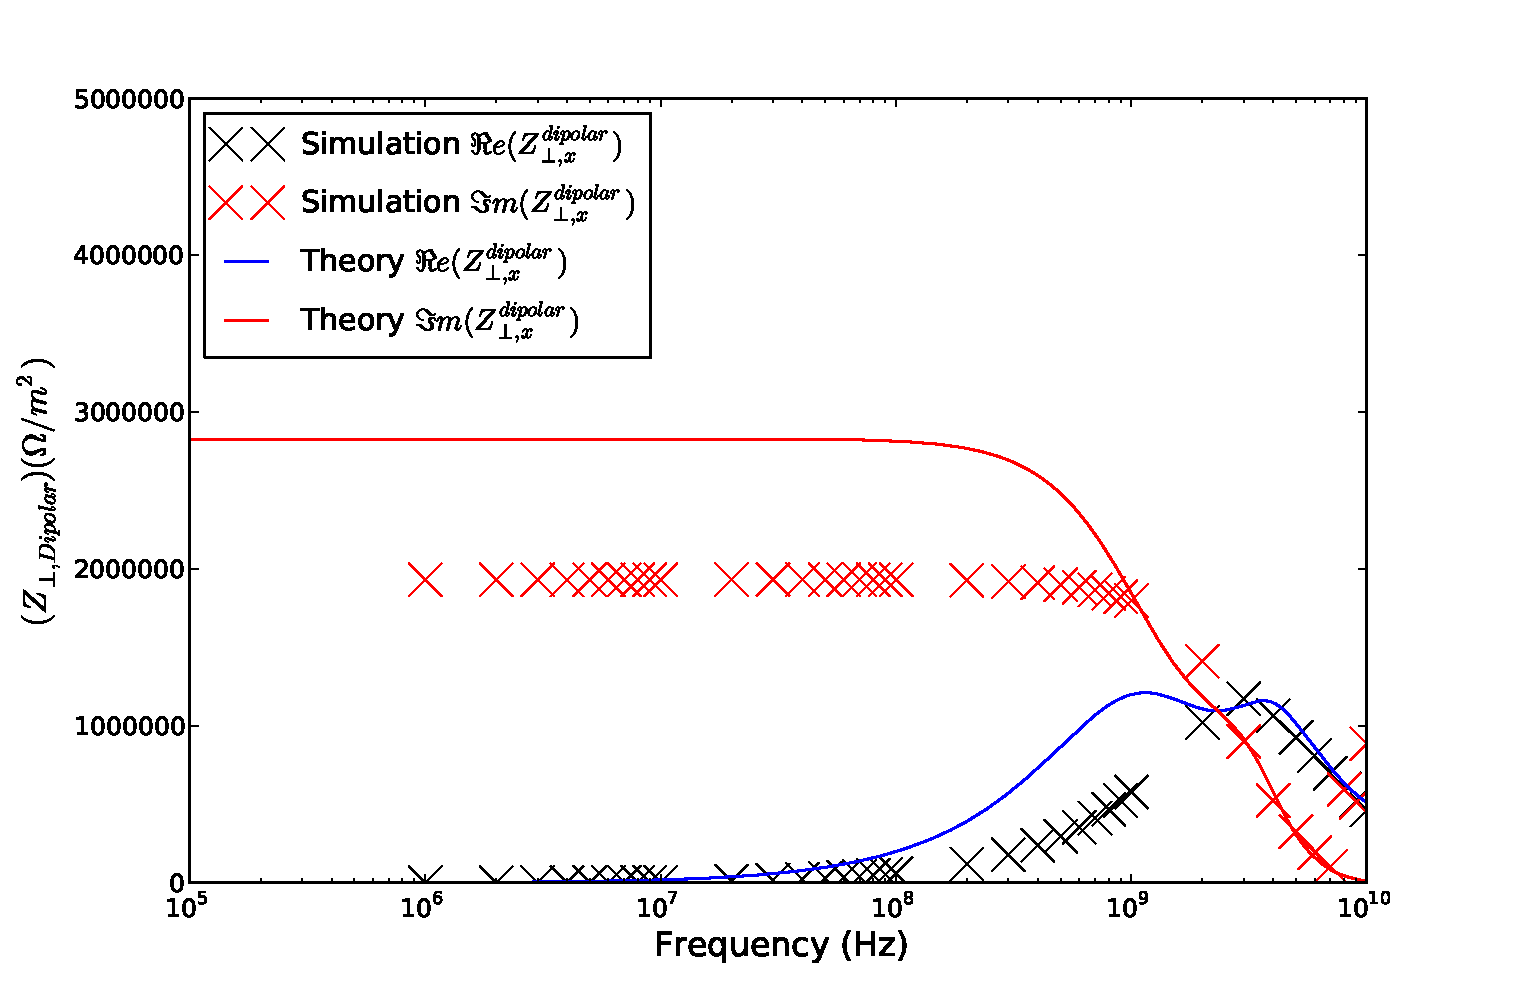
\includegraphics[width=0.5\textwidth]{figures/wire_meas/ferrite_plates/dipolar-horizontal.pdf}
\label{fig:ferrite-plates-dip-horz}
}
\subfigure[]{
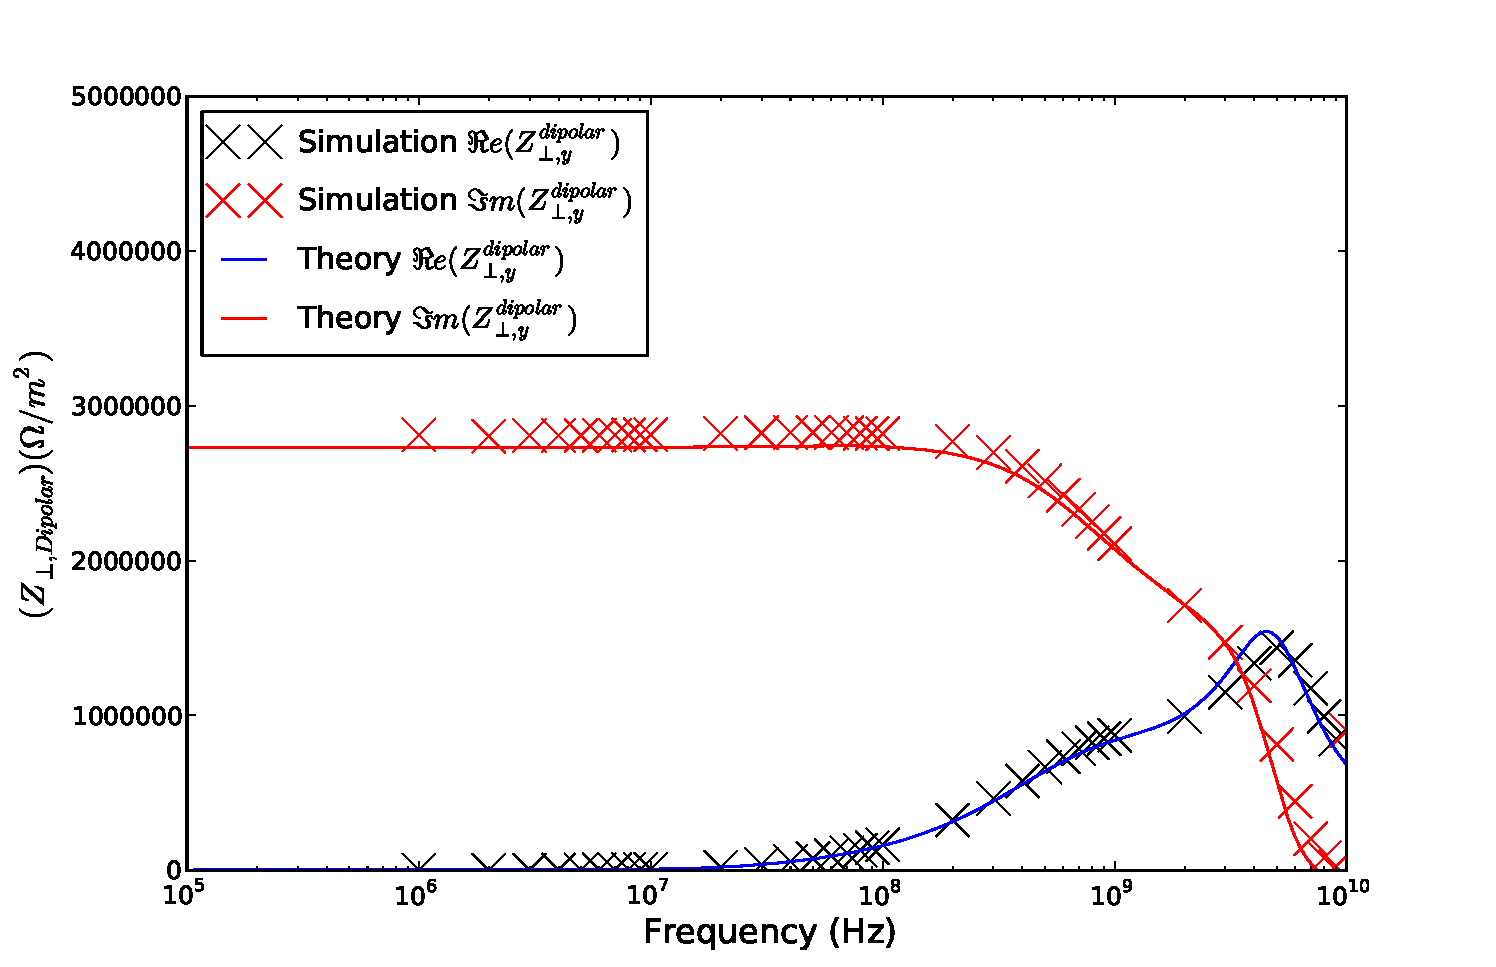
\includegraphics[width=0.5\textwidth]{figures/wire_meas/ferrite_plates/dipolar-vertical.pdf}
\label{fig:ferrite-plates-dip-vert}
}
\caption{The dipolar impedance of two parallel ferrite plates simulated using two longitudinal coaxial wires. Presented are is the impedance as measured in the horizontal plane (\ref{fig:ferrite-plates-dip-horz}) and in the vertical plane \ref{fig:ferrite-plates-dip-vert}.}
\label{fig:ferrite-plates-dipolar}
\end{figure}

\begin{figure}
\subfigure[]{
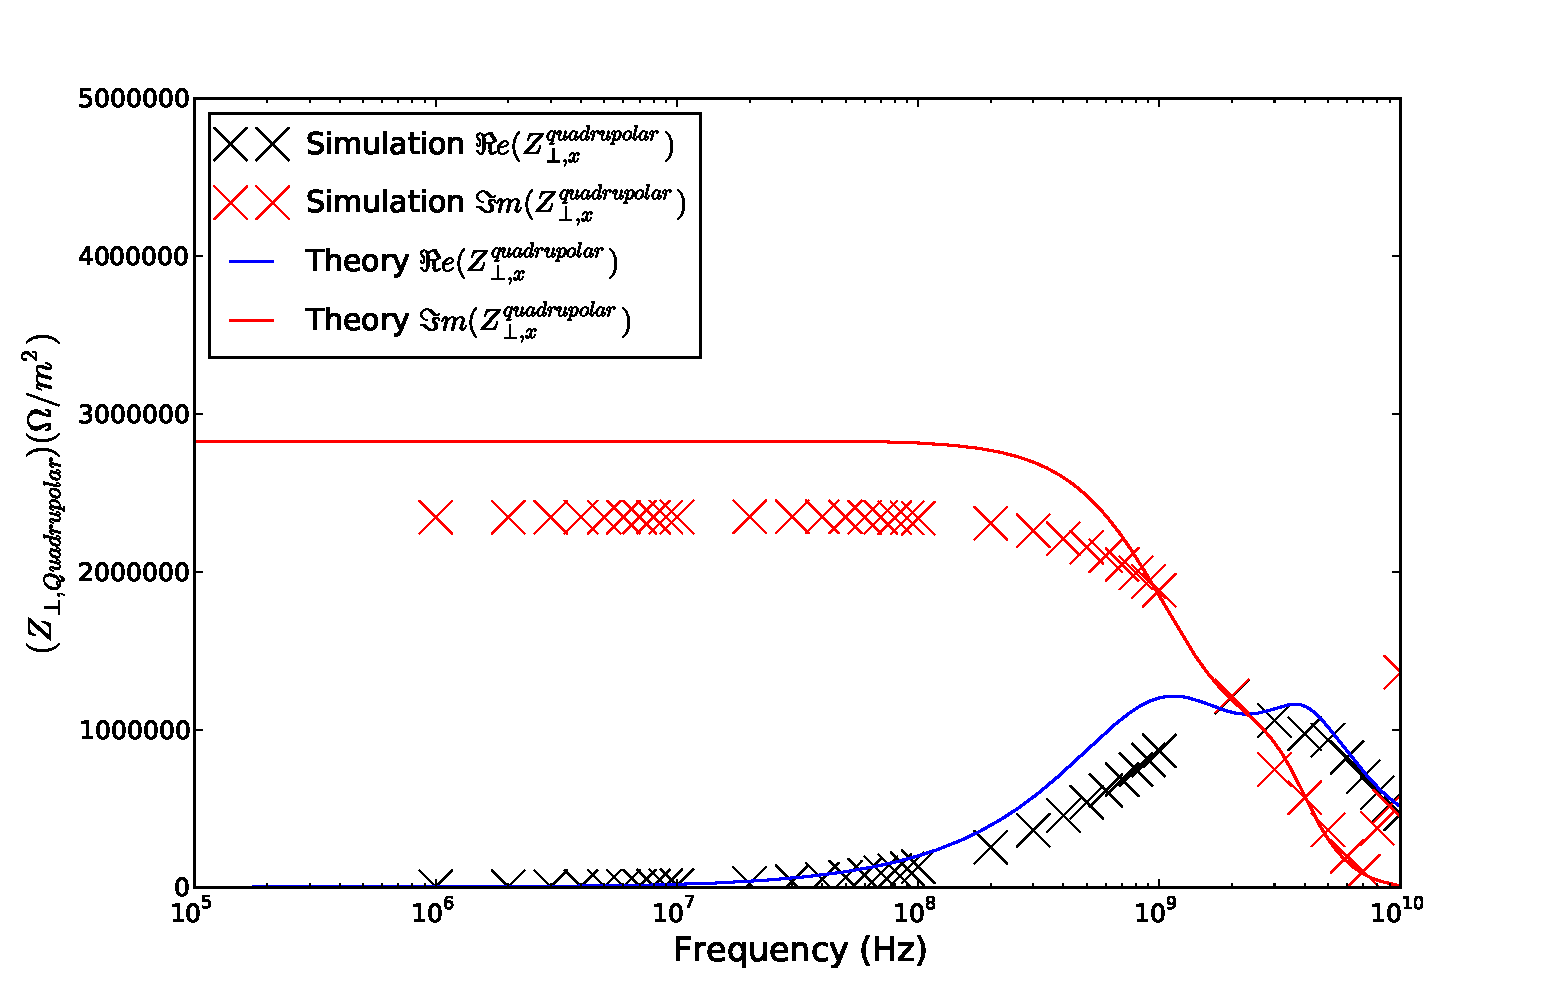
\includegraphics[width=0.5\textwidth]{figures/wire_meas/ferrite_plates/quadrupolar-horizontal.pdf}
\label{fig:ferrite-plates-quad-horz}
}
\subfigure[]{
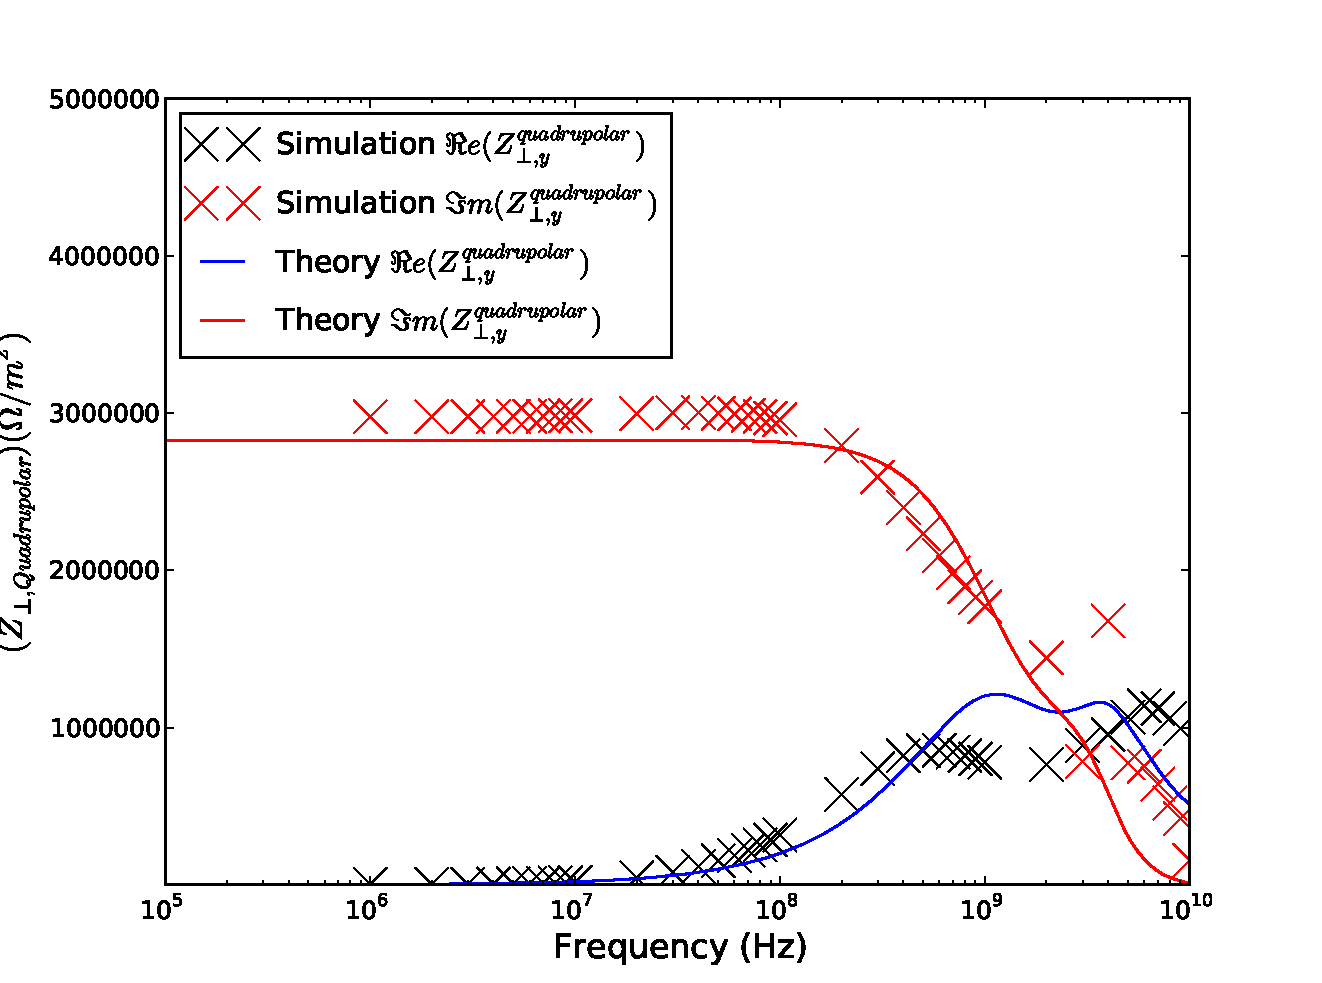
\includegraphics[width=0.5\textwidth]{figures/wire_meas/ferrite_plates/quadrupolar-vertical.pdf}
\label{fig:ferrite-plates-quad-vert}
}
\caption{The quadrupolar impedance of two parallel ferrite plates simulated using a combination of displaced single wire simulated measurements and two wire simulated mesurements. Presented are is the impedance as measured in the horizontal plane (\ref{fig:ferrite-plates-quad-horz}) and in the vertical plane \ref{fig:ferrite-plates-quad-vert}.}
\label{fig:ferrite-plates-quadrupolar}
\end{figure}

The longitudinal impedance is as determined by taking the constant term for a series of simulated displaced wire measurements in both the vertical and horizontal planes is shown in Fig.~\ref{fig:ferrite-plates-long}. It can be seen that in the frequency range below 100MHz the agreement between the coaxial wire results and the analytical results is very good in both the vertical and horizontal plane. Above 100MHz the agreement for the real components is very good for both results, however the imaginary component in the vertical plane displays some substantial disagreement. This is likely due to the high mesh density required to correctly evaluate the phase change along the length of the simulated structure. A higher mesh density may correct this, however limits of computational resource presently make this unfeasible.

The agreement between the simulations of the vertical dipolar impedance and the theoretical model is excellent across all frequencies for both the real and imaginary components. The agreement below 100MHz and above 1GHz is very good for the horizontal dipolar, with some divergence in the constant term of the imaginary impedance. The key difference is the failure of the coaxial method to resolve one of the peaks in the real impedance. The results for the dipolar impedance are shown in Fig.~\ref{fig:ferrite-plates-dipolar}.

The results for the quadrupolar impedance are shown in Fig.~\ref{fig:ferrite-plates-quadrupolar}. The vertical simulations agree well with the theory, correctly identifying the two peaks in the quadrupolar impedance. The agreement for the horizontal simulations with theory is less good. This can be explained by the derivation of the horizontal quadrupolar being highly dependent on the quality of the horizontal dipolar impedance results due to them cancelling each other to form the total transverse impedance. As the horizontal dipolar impedance does not resolve the the subpeaks neither does the horizontal quadrupolar impedance calculations.

\section{The Impedance of a Displaced Coaxial Wire in an Asymmetric Device}
\label{sec:AsymMath}

If Eqn. \ref{eqn:gen_single_wire} is transformed from $\left( x,y \right)$ coordinates to $\left( a, \theta \right)$, the result is

\begin{align}
Z &=Z_{0,0} +a\left[ cos\theta \left( Z_{-1,0} + Z_{0,1} \right) +jsin\theta \left( Z_{-1,0} + Z_{0,1} \right)  cos\theta \left( Z_{1,0} + Z_{0,-1} \right) - jsin\theta \left( Z_{1,0} + Z_{0,-1} \right)\right] \nonumber \\
   &+a^{2}\left[ cos^{2} \left( Z_{1,1} + Z_{-1,-1} \right) + sin^{2} \left( Z_{1,1} + Z_{-1,-1} \right)\right] \nonumber \\
   &+a^{2}\left[ cos^{2} \left( Z_{2,0} + Z_{0,-2} +Z_{1,-1} \right) +2jsin\theta cos\theta\left( Z_{2,0} + Z_{0,-2} +Z_{1,-1} \right) \right] \nonumber \\
   & - a^{2}\left[sin^{2} \left( Z_{2,0} + Z_{0,-2} +Z_{1,-1} \right)\right] \nonumber  \\
   &+ a^{2}\left[ cos^{2} \left( Z_{-2,0} + Z_{0,2} +Z_{-1,1} \right) +2jsin\theta cos\theta\left( Z_{-2,0} + Z_{0,2} +Z_{-1,1}  \right) \right] \nonumber \\
   &+ a^{2}\left[sin^{2} \left( Z_{-2,0} + Z_{0,2} +Z_{-1,1}  \right) \right].
\end{align}

Grouping like terms this becomes
\begin{align}
Z   &=Z_{0,0} + a\left[ e^{-j\theta}\left( Z_{-1,0} + Z_{0,1} \right) +  e^{j\theta}\left( Z_{1,0} + Z_{-0,1} \right)\right] \nonumber \\
     &+a^{2}\left[ \left( Z_{1,1} + Z_{-1,-1} \right) + e^{-2j\theta} \left(  Z_{2,0} + Z_{0,-2} +Z_{1,-1} \right) + e^{2j\theta} \left( Z_{-2,0} + Z_{0,2} +Z_{-1,1} \right) \right] \nonumber \\
     &=A_{1} + ae^{-j\theta}A_{2} + ae^{-j\theta}A_{3}+ a^{2}e^{-2j\theta}A_{4} +a^{2}e^{2j\theta}A_{5} +  a^{2}A_{6}
\label{eqn:rot_gen}
\end{align}

where $A_{1} = Z_{0,0}$, $A_{2} = Z_{0,1}+Z_{-1,0}$, $A_{3} = Z_{0,-1}+Z_{1,0}$, $A_{4} = Z_{0,2}+Z_{-1,1}+Z_{-2,0}$, $A_{5} = Z_{2,0}+Z_{1,-1}+Z_{0,-2}$ and $A_{6}=Z_{1,1}+Z_{-1,-1}$. Taking the earlier definition of $Z_{quad}$ it can be deduced that

\begin{align}
Z_{quad} & = \left( A_{4}+A_{5}+A_{6} - \bar{Z}_{x} \right)\frac{1}{k} =\frac{ A_{4}+A_{5}+A_{6}}{k} - Z^{dip}_{x} \\  
	    & = \left( A_{4}+A_{5} - \frac{\bar{Z}_{x}- \bar{Z}_{y}}{2}\right)\frac{1}{k} =\frac{ A_{4}+A_{5}}{k} - \frac{Z^{dip}_{x}-Z^{dip}_{y} }{2}.
\end{align}

Consideration of Eqn. \ref{eqn:rot_gen} lets it be seen that

\begin{align}
 A_{4}+A_{5}+A_{6} & = \frac{Z\left( a,0 \right)+Z\left( a,\pi \right) - 2Z\left( 0,0 \right)}{2a^{2}} \\
 A_{4}+A_{5} & = \frac{Z\left( a,0 \right)+Z\left( a,\pi \right) - Z\left( a,\frac{\pi}{2} \right)-Z\left( a,\frac{3\pi}{2} \right)}{2a^{2}}.
\end{align}

The constant impedance can also be seen to be found by taking a linear fit of the longitudinal impedance of a wire displaced in either the $\theta = 0$ or $\theta = \pi / 2$ plane, and taking the linear term of the fit. 

\section{Simulated Measurements of Coaxial Wire Technique in a C-Core Kicker}
\label{sec:AsymSims}

To test the measurement method for an asymmetric structure a model of the c-core ferrite kicker magnet was used, as shown in Fig.\ref{fig:zannini-model}, the analytical details of which are given in \cite{Zannini:cCoreFerrite}. Key in this type of structure is that it predictsa non-zero constant transverse impedance term as well as the quadrupolar terms, thus we may completely evaluate the asymmetric measurement method. For these simulations a structure of $a=15$mm, $r=20$mm, $\theta = \pi / 2$, and $100$mm in length was used. Simulations were carried out using the classical coaxial wire method as simulated in HFSS.

The following parameters were used for the simulations; wire of 0.2mm in radius, and the following displacement used to acquire the total transverse terms:

\begin{enumerate}
\item{In the horizontal axis -  displaced between -5mm to +5mm at intervals of 1mm}
\item{In the vertical axis - displaced between -5mm to +5mm at intervals of 1mm.}
\end{enumerate}

For the two wire simulations, two wires of radius 0.2mm are modelled, with a seperation of 2mm in the x-dimension, and 2mm in the y-dimension. Four simulation configurations are used described below:

\begin{enumerate}
\item{an adaptive mesh generation set to a convergence criteria of $S_{21}$ diverging by less than 0.005 between two subsequent solutions, at an adaptive frequency of 20MHz solving to a second order basis. A discrete frequency sweep is then carried out in the range 1-10MHz at 1MHz intervals.}
\item{an adaptive mesh generation set to a convergence criteria of $S_{21}$ diverging by less than 0.005 between two subsequent solutions, at an adaptive frequency of 200MHz solving to a second order basis. A discrete frequency sweep is then carried out in the range 10-100MHz at 10MHz intervals.}
\item{an adaptive mesh generation set to a convergence criteria of $S_{21}$ diverging by less than 0.005 between two subsequent solutions, at an adaptive frequency of 2GHz solving to a second order basis. A discrete frequency sweep is then carried out in the range 100MHz-1GHz at 100MHz intervals.}
\item{an adaptive mesh generation set to a convergence criteria of $S_{21}$ diverging by less than 0.005 between two subsequent solutions, at an adaptive frequency of 10GHz solving to a second order basis. A discrete frequency sweep is then carried out in the range 1-10GHz at 1GHz intervals.}
\end{enumerate}

These parameters are used to benefit from an appropriate mesh count for the given frequency range, thus increasing simulation speed by not using a high density mesh at frequencies where no benefits would be gained.

\begin{figure}
\subfigure[]{
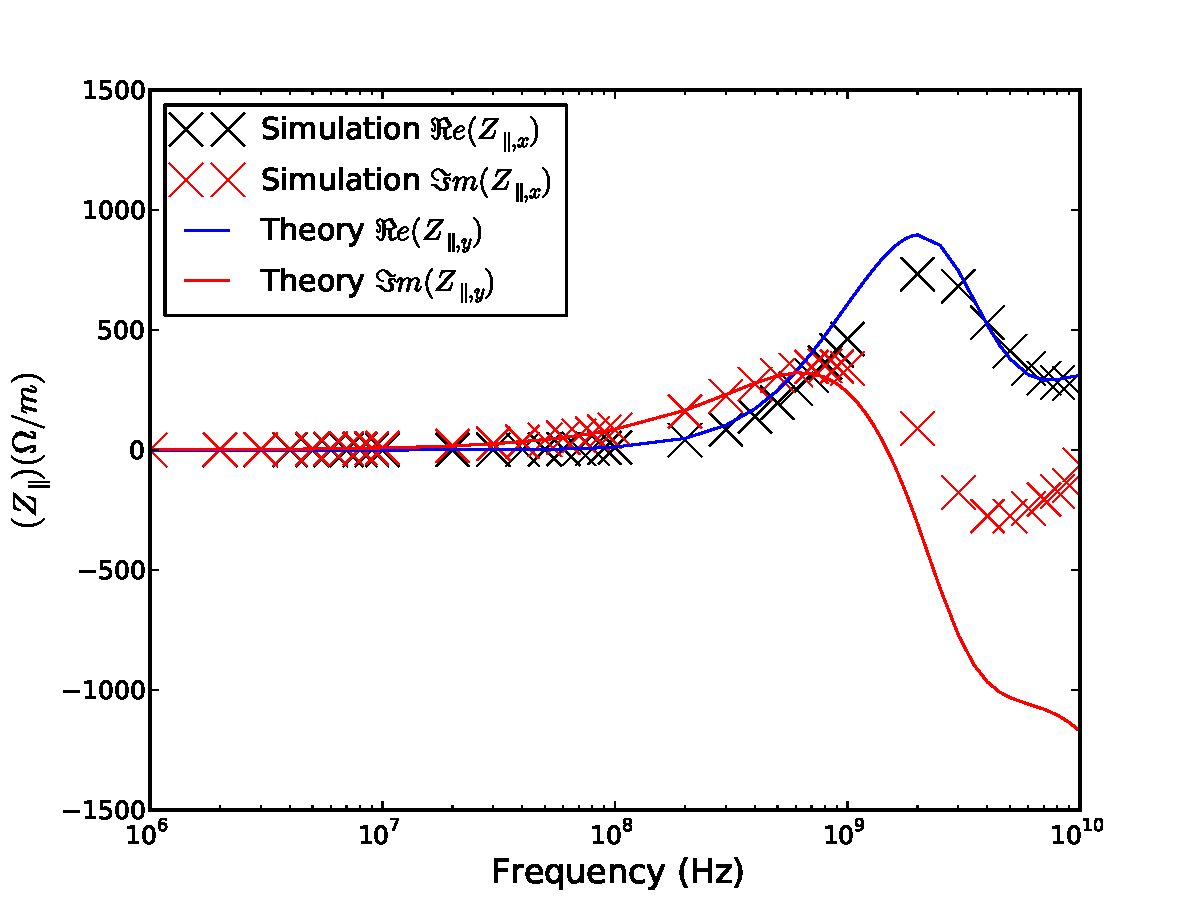
\includegraphics[height=0.35\textwidth]{figures/wire_meas/ferrite-c-core/longitudinal-impedance.pdf}
\label{fig:c-core-longitudinal}
}
\subfigure[]{
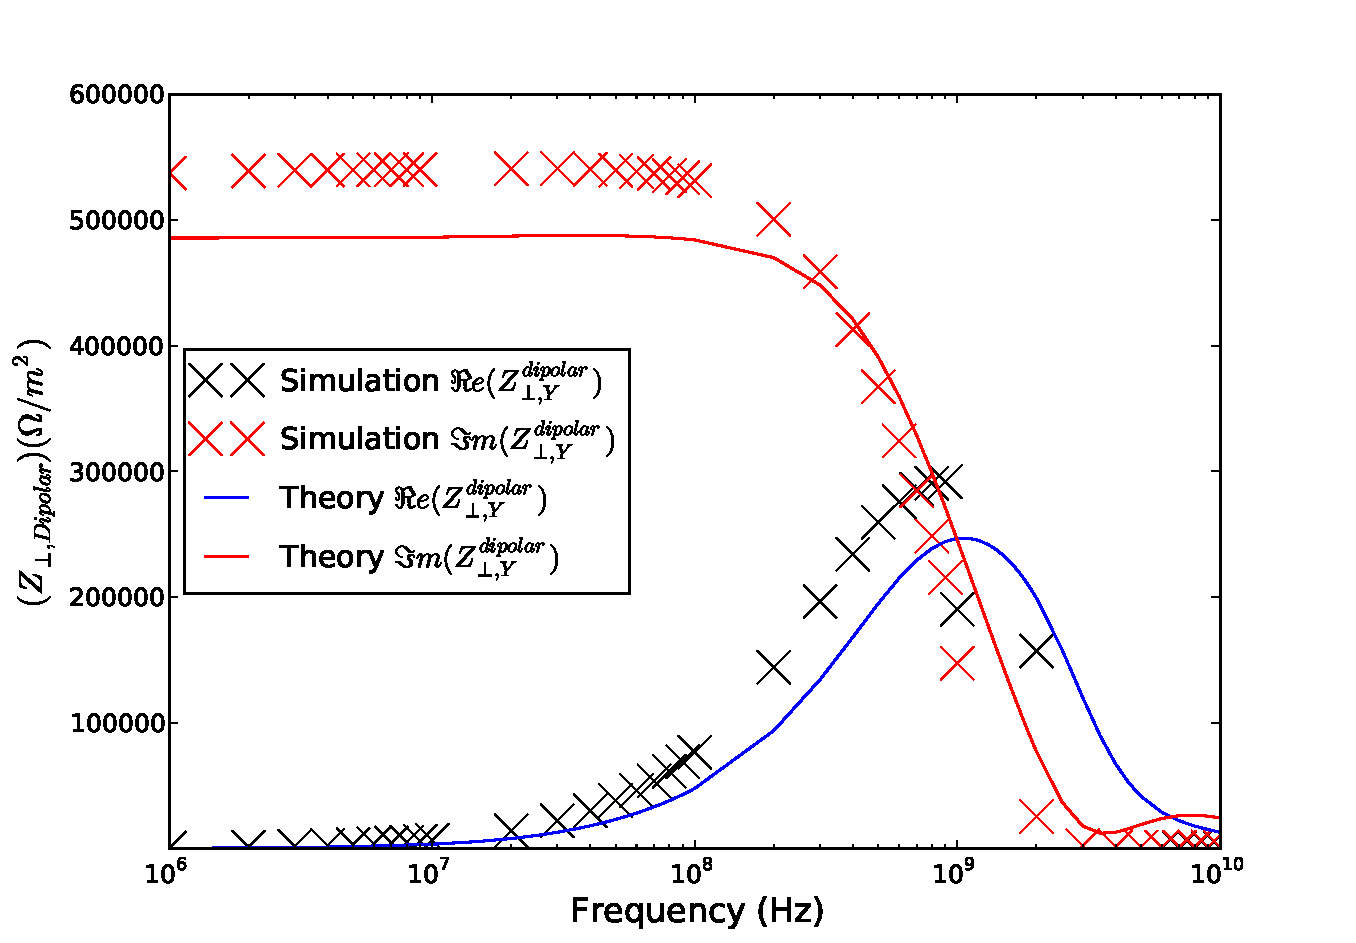
\includegraphics[height=0.35\textwidth]{figures/wire_meas/ferrite-c-core/dipolar-vertical-impedance.pdf}
\label{fig:c-core-dipolar}
}
\subfigure[]{
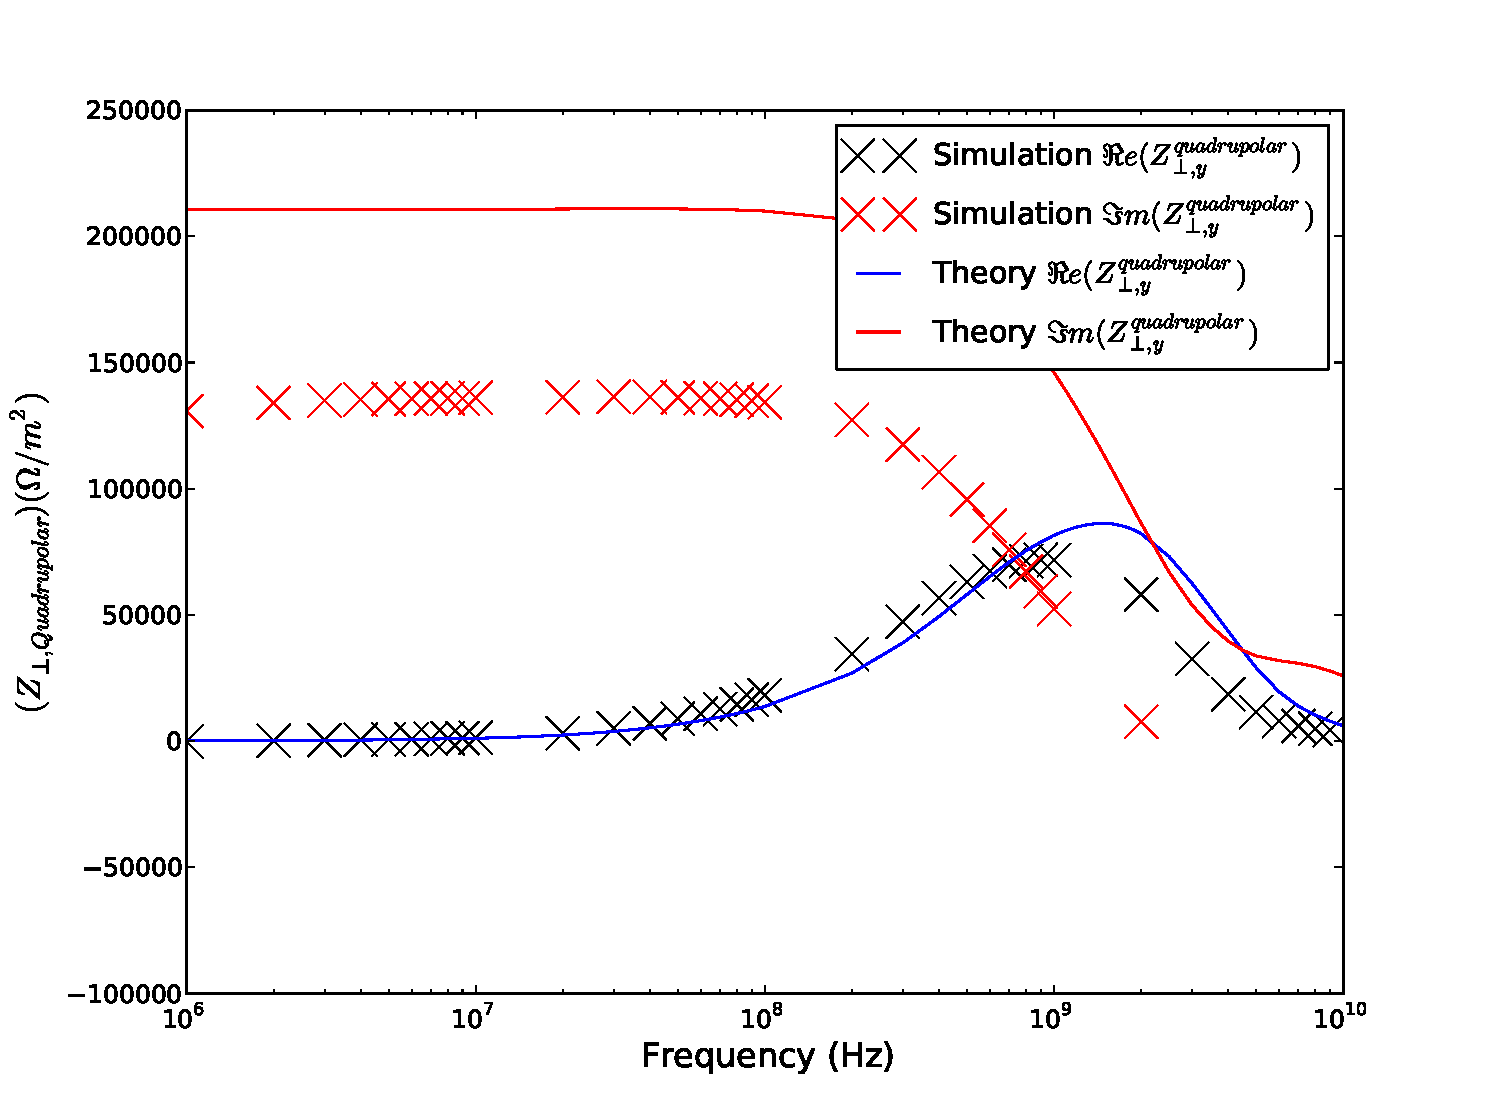
\includegraphics[height=0.35\textwidth]{figures/wire_meas/ferrite-c-core/quadrupolar-vertical-impedance.pdf}
\label{fig:c-core-quadrupolar}
}
\subfigure[]{
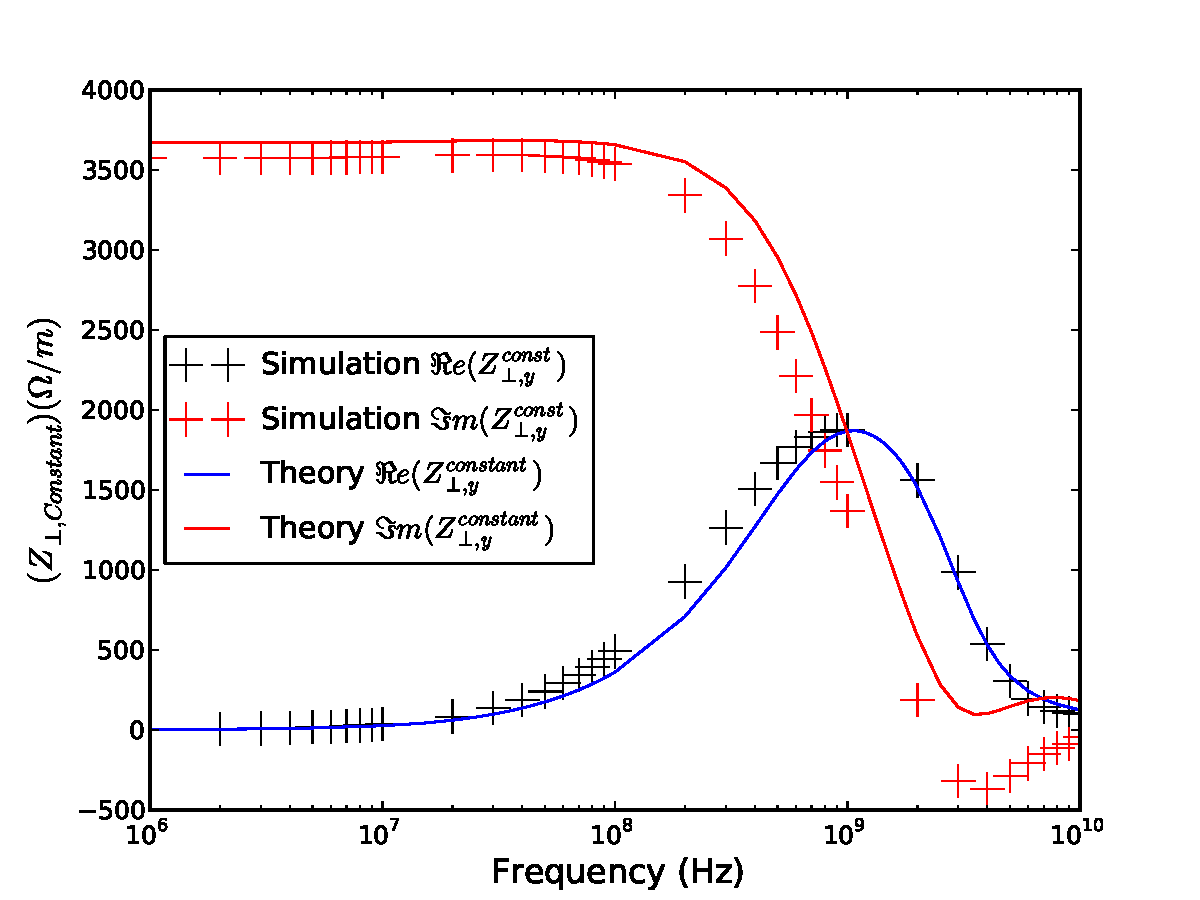
\includegraphics[height=0.35\textwidth]{figures/wire_meas/ferrite-c-core/constant-vertical-impedance.pdf}
\label{fig:c-core-constant}
}
\caption{The impedance of the c-core ferrite kicker as acquired by simulating the classical coaxial wire method in HFSS. Shown is the \ref{fig:c-core-longitudinal} longitudinal impedance, \ref{fig:c-core-dipolar} the dipolar impedance, \ref{fig:c-core-quadrupolar} the quadrupolar impedance and \ref{fig:c-core-constant} the constant transverse impedance.}
\end{figure}

It can be seen that the longitudinal impedance agrees well over the entire frequency range below 1GHz (Fig.~\ref{fig:c-core-longitudinal}). The analytical calculations breakdown above 1GHz due to the family of Bessel functions used for the calculations being optimised for low frequency calculations. Similarly the agreement for the dipolar impedance can be seen to be exceptionally good over the majority of the frequency range, with an increasing descrepency at high frequencies (Fig.~\ref{fig:c-core-dipolar}).

To test the asymmetric method we should look at the constant and quadrupolar terms. In this case it can be seen that the agreement with the constant transverse term is exceptionally good across the entire frequency range (Fig.~\ref{fig:c-core-constant}). The agreement for the quadrupolar impedance is good in the range of frequencies below 1GHz. Above this the unsuitability of the family of Bessel functions used for this frequency range becomes more apparents and the simulated and analytical results diverge.

It can be seen that the proposed asymmetric method can replicate the beam coupling impedance of an asymmetric structure, correctly predicting both longitudinal and transverse (dipolar, quadrupolar and constant) terms below 1GHz. 



\section{Summary}
\label{sec:ConSum}

\bibliographystyle{elsarticle-num}
\bibliography{coaxWireMeasBib}

\end{document}
